%%%%%%%%%%%%%%%%%%%%%%%%%%%%%%%%%%%%%%%%%%%%%%%%%%%%%%%%%%%%%%%%%%%%%%%%%%%%%%%%%%
\begin{frame}[fragile]\frametitle{}
\begin{center}
{\Large Notes from Samkhya Darshan}
\end{center}
\end{frame}

%%%%%%%%%%%%%%%%%%%%%%%%%%%%%%%%%%%%%%%%%%%%%%%%%%%%%%%%%%%
\begin{frame}[fragile]\frametitle{भारतीय दर्शन का परिचय}
      \begin{itemize}
	\item भारतीय दर्शन जीवन और ब्रह्मांड के रहस्यों को सुलझाने का अनूठा प्रयास है.
	\item दर्शन का अर्थ केवल फिलॉसफी नहीं बल्कि देखना या अनुभव करना भी है. यह वह ज्ञान है जो ऋषियों ने गहरे चिंतन और अनुभव से प्राप्त किया.
    \item मनुष्य की हमेशा से जिज्ञासा रही है की हमारा अस्तित्व आया कहां से? हमारे अतीत का कारण क्या है? ब्रह्मांड की उत्पत्ति हुई कहां से? जो हमारी ऋषि मुनि हुए उनको भी यह सब समझना था.
	\item षड्दर्शन में छ: प्रमुख दर्शन हैं - न्याय, वैशेषिक, सांख्य, योग, मीमांसा और वेदांत.
	\item यह सभी वेदों को मानते हैं इसलिए इन्हें आस्तिक दर्शन कहा जाता है.
    \item सनातन धर्म के केंद्र में जो चार वेद है ऋग्वेद यजुर्वेद सामवेद अथर्ववेद और उनके भाग, आरण्यक, ब्राह्मण , संहिता , उपनिषद. इनके आधार पर जब ऋषि मुनियों ने अध्ययन किया तो छह दर्शन मानव जीवन को समझने के लिए दिये, उसमेसे एक है सांख्य दर्शन.
    \item ढेर सारे मजहब बताते हैं की सृष्टि को किसी ईश्वर ने बना दिया है. इस धार्मिक विचार से हटकर हमारे ऋषि मुनियों ने दी और जो बहुत तार्किक को शास्त्रीय हो, वो है, सांख्य दर्शन.
	  \end{itemize}
\end{frame}

%%%%%%%%%%%%%%%%%%%%%%%%%%%%%%%%%%%%%%%%%%%%%%%%%%%%%%%%%%%
\begin{frame}[fragile]\frametitle{सांख्य दर्शन: अर्थ एवं महत्व}
  \begin{itemize}
	\item सांख्य दर्शन को भारतीय चिंतन का आधार स्तंभ माना जाता है.
    \item सांख्य शब्द संख्या से बना है जिसका अर्थ है गिनती या गणना करना. यह सृष्टि के मूल तत्वों की सटीक गणना करता है.
    \item इसका दूसरा अर्थ विवेकपूर्ण ज्ञान भी है. यह हमें सत्य और असत्य, आत्मा और अनात्मा के बीच भेद करना सिखाता है.
	\item यह सिखाता है कि यह दुनिया कैसे बनी और हम कौन हैं, हमें दुख क्यों होता है और इससे हमेशा के लिए छुटकारा कैसे मिले.
	\item यह सृष्टि और चेतना के रहस्य को दो मूल तत्वों - पुरुष और प्रकृति के माध्यम से समझाता है.
    \item इसके सिद्धांतों का प्रभाव योग, वेदांत, आयुर्वेद और भगवत गीता में भी दिखाई देता है.
  \end{itemize}
\end{frame}

%%%%%%%%%%%%%%%%%%%%%%%%%%%%%%%%%%%%%%%%%%%%%%%%%%%%%%%%%%%%%%%%%%%%%%%%%%%%%%%%%%
\begin{frame}[fragile]\frametitle{प्रवर्तक एवं मुख्य ग्रंथ}
\begin{columns}
    \begin{column}[T]{0.6\linewidth}
      \begin{itemize}
        \item परंपरागत रूप से सांख्य दर्शन के प्रणेता महर्षि कपिल माने जाते हैं, जिन्हें अत्यंत प्राचीन और सिद्ध ऋषि माना जाता है.
        \item उनका मूल ग्रंथ \textbf{सांख्य प्रवचन सूत्र (Sāṅkhya Pravacana Sūtra)} माना जाता है, जो आज अपने मूल रूप में मिलता ही नहीं है.
        \item वर्तमान में प्रमुख और सबसे प्राचीन उपलब्ध ग्रंथ \textbf{सांख्य कारिका (Sāṅkhya Kārikā)} है.
        \item इसके रचयिता ईश्वरकृष्ण (Īśvarakṛṣṇa) हैं. यह 72 सूत्रों में दर्शन की पूर्ण प्रस्तुति है.
        \item कारिका पर अनेक टीकाएँ हैं, जैसे गौड़पाद, वाचस्पति मिश्र आदि द्वारा.
      \end{itemize}
    \end{column}
    \begin{column}[T]{0.4\linewidth}
      \begin{center}
        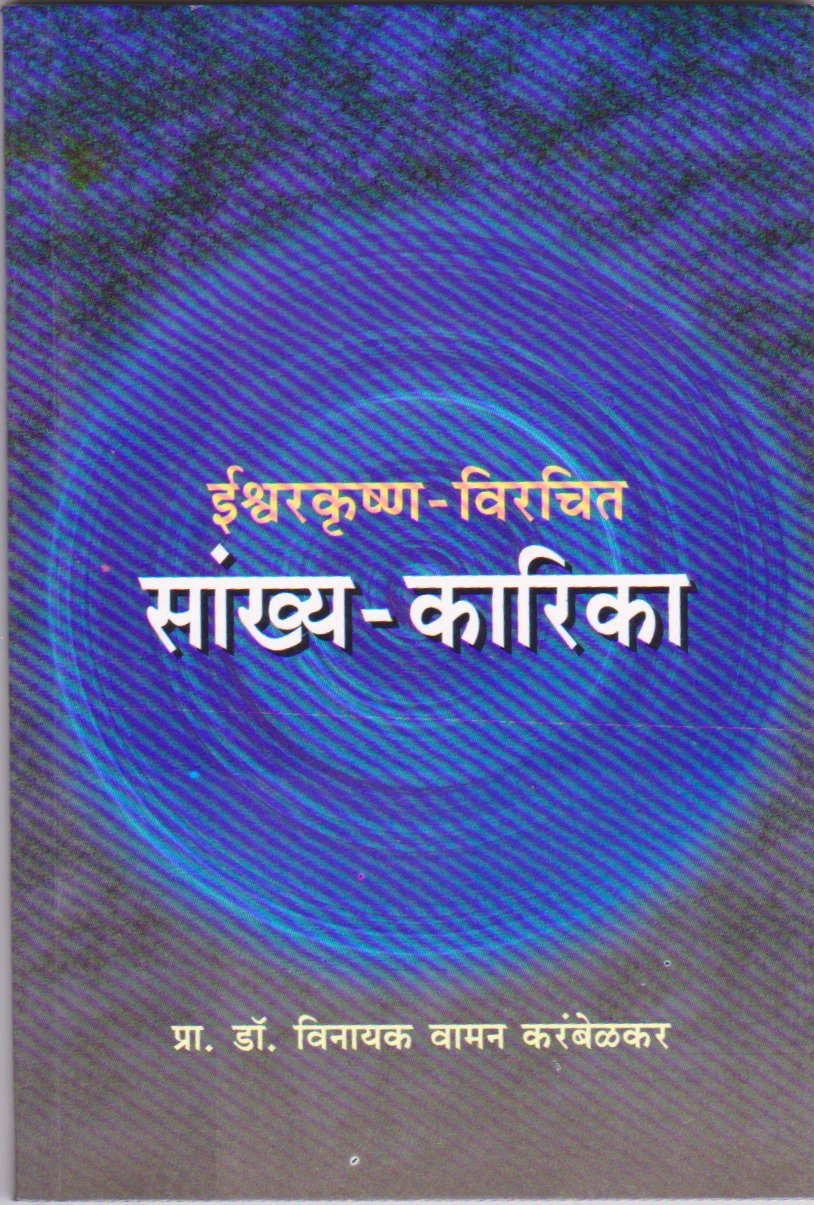
\includegraphics[width=\linewidth,keepaspectratio]{sankhya3}
      \end{center}	
    \end{column}
\end{columns}
\end{frame}

%%%%%%%%%%%%%%%%%%%%%%%%%%%%%%%%%%%%%%%%%%%%%%%%%%%%%%%%%%%
\begin{frame}[fragile]\frametitle{मूल सिद्धांत: द्वैतवाद एवं अनीश्वरवाद}
      \begin{itemize}
	\item सांख्य दर्शन की सबसे बड़ी विशेषता इसका द्वैतवाद है. सृष्टि के मूल में दो स्वतंत्र, अनादि और अनंत सत्ताएं हैं.
        \begin{itemize}
            \item पहली सत्ता: पुरुष - चेतना, आत्मा या ज्ञाता.
            \item दूसरी सत्ता: प्रकृति - जड़ पदार्थ, ऊर्जा या अचेतन मूल तत्व.
        \end{itemize}
	\item यह संख्या दर्शन अनीश्वरवादी (agnostic) है. यह ईश्वर को सृष्टिकर्ता नहीं मानता.
	\item यह ईश्वर को भले न नाकारती हो लेकिन यह भी नहीं मानती की ईश्वर ने सृष्टि की रचना की होगी.
	\item फिर भी यह \textbf{आस्तिक} (Āstika) दर्शन है, क्योंकि यह वेदों को प्रमाण मानता है.
	  \end{itemize}
\end{frame}

%%%%%%%%%%%%%%%%%%%%%%%%%%%%%%%%%%%%%%%%%%%%%%%%%%%%%%%%%%%
\begin{frame}[fragile]\frametitle{पुरुष: चेतना का सिद्धांत}
      \begin{itemize}
	\item पुरुष (Puruṣa) शुद्ध चेतना है. उसका स्वभाव ही चेतन है - वह जानने वाला, देखने वाला (दृष्टा) और अनुभव करने वाला (भोक्ता) है.
    \item चेतना का अर्थ है अनुभव करना - यही पुरुष का मूल कार्य है.
	\item यद्यपि वह ज्ञाता और भोक्ता है, वह स्वयं निष्क्रिय (अकर्ता) है और केवल एक साक्षी (विटनेस) की तरह प्रकृति के खेल को देखता है.
	\item वह निर्गुण, अक्रिय, और साक्षी रूप है. वह सुख-दुख, पाप-पुण्य, जन्म-मरण से परे है.
	\item पुरुष में कोई परिवर्तन नहीं होता - वह निर्विकार है.
	\item सांख्य की महत्वपूर्ण मान्यता: पुरुष अनेक हैं. हर जीव में एक अलग पुरुष (चेतना) वास करती है.
    \item इसीलिए हर जीव का अनुभव (सुख-दुख, जन्म-मरण, मोक्ष) अलग-अलग होता है.
    \item पुरुष के अस्तित्व का तर्क: सारी सृष्टि जो जड़ प्रकृति से बनी है, किसी चेतन पुरुष के भोग और मोक्ष के लिए है.
	  \end{itemize}
\end{frame}

%%%%%%%%%%%%%%%%%%%%%%%%%%%%%%%%%%%%%%%%%%%%%%%%%%%%%%%%%%%
\begin{frame}[fragile]\frametitle{प्रकृति: जड़ जगत का मूल कारण}
      \begin{itemize}
	\item प्रकृति (Prakṛti) ब्रह्मांड का उपादान कारण (material cause) है. उसे प्रधान भी कहा जाता है क्योंकि वही सभी कार्यों का मूल कारण है.
    \item उसे अव्यक्त भी कहते हैं क्योंकि अपनी मूल अवस्था में वह प्रकट नहीं होती. वह अज (Unborn) और अनादि (Eternal) है.
	\item प्रकृति अपने स्वभाव से अचेतन (जड़) है; उसमें अपनी कोई चेतना या बुद्धि नहीं होती.
	\item इसके विपरीत प्रकृति अत्यंत सक्रिय है. सारा बदलाव, सारी गति, सारा कार्य प्रकृति में ही संभव होता है.
	\item जहां पुरुष अनेक माने गए हैं, वहीं प्रकृति केवल एक ही है.
	\item प्रकृति की सबसे महत्वपूर्ण विशेषता: वह त्रिगुणात्मिका है, यानी तीन गुणों या शक्तियों से बनी है.
    \item प्रकृति के अस्तित्व का तर्क: यह व्यक्त जगत एक कार्य है, इसलिए इसका कोई अव्यक्त कारण होना चाहिए - वही प्रकृति है.
	  \end{itemize}
\end{frame}

%%%%%%%%%%%%%%%%%%%%%%%%%%%%%%%%%%%%%%%%%%%%%%%%%%%%%%%%%%%
\begin{frame}[fragile]\frametitle{प्रकृति के तीन गुण: सत्व, रजस और तमस}
      \begin{itemize}
	\item \textbf{सत्वगुण}: प्रकाश, ज्ञान, सुख, शांति, हल्कापन और अच्छाई का प्रतीक. मन में स्थिरता, निर्मलता और प्रसन्नता लाता है. प्रतीकात्मक रंग सफेद है.
	\item \textbf{रजसगुण}: क्रिया, गति, बेचैनी, इच्छा, दुख और ऊर्जा का प्रतिनिधित्व करता है. हमें कर्म करने के लिए प्रेरित करता है लेकिन अशांति का कारण भी बनता है. इसका रंग लाल है.
	\item \textbf{तमसगुण}: अंधकार, अज्ञान, आलस्य, मोह और भारीपन का द्योतक है. ज्ञान को ढकता है और हमें निष्क्रिय बनाता है. प्रतीकात्मक रंग काला है.
    \item यह तीनों गुण हमेशा एक साथ रहते हैं जैसे एक रस्सी के तीन धागे आपस में गूंथे होते हैं.
	\item इन्हीं गुणों के विभिन्न अनुपातों में मिलने से दुनिया की सारी विविधता पैदा होती है.
    \item जब सृष्टि नहीं होती (प्रलय की अवस्था) तब तीनों गुण पूर्ण साम्य अवस्था में रहते हैं.
	  \end{itemize}
\end{frame}

%%%%%%%%%%%%%%%%%%%%%%%%%%%%%%%%%%%%%%%%%%%%%%%%%%%%%%%%%%%%%%%%%%%%%%%%%%%%%%%%%%
\begin{frame}[fragile]\frametitle{सत्कार्यवाद: कार्यकारण सिद्धांत}
\begin{columns}
    \begin{column}[T]{0.6\linewidth}
      \begin{itemize}
		\item सांख्य का अत्यंत महत्वपूर्ण दार्शनिक सिद्धांत है सत्कार्यवाद.
		\item इसका अर्थ है कि कार्य (effect) अपनी उत्पत्ति से पहले ही अपने कारण (cause) में अव्यक्त रूप में मौजूद रहता है. For effect there has to be a cause.
        \item सृष्टि में कुछ भी बिल्कुल नया उत्पन्न नहीं होता. जो पहले से ही कारण में बीज रूप में विद्यमान था, वही प्रकट हो जाता है.
        \item "शून्य से कुछ नहीं बनता" — यह \textbf{असत्कार्यवाद} का खंडन है.
        \item उदाहरण: दूध ही दही में परिवर्तित होता है, पानी से दही नहीं बन सकता. तिल में तेल पहले से ही विद्यमान होता है, उसे केवल निकालकर प्रकट किया जाता है.
        \item कारण के दो प्रकार: \textbf{निमित्त} (Nimitta) और \textbf{उपादान} (Upādāna).
      \end{itemize}
    \end{column}
    \begin{column}[T]{0.4\linewidth}
      \begin{center}
        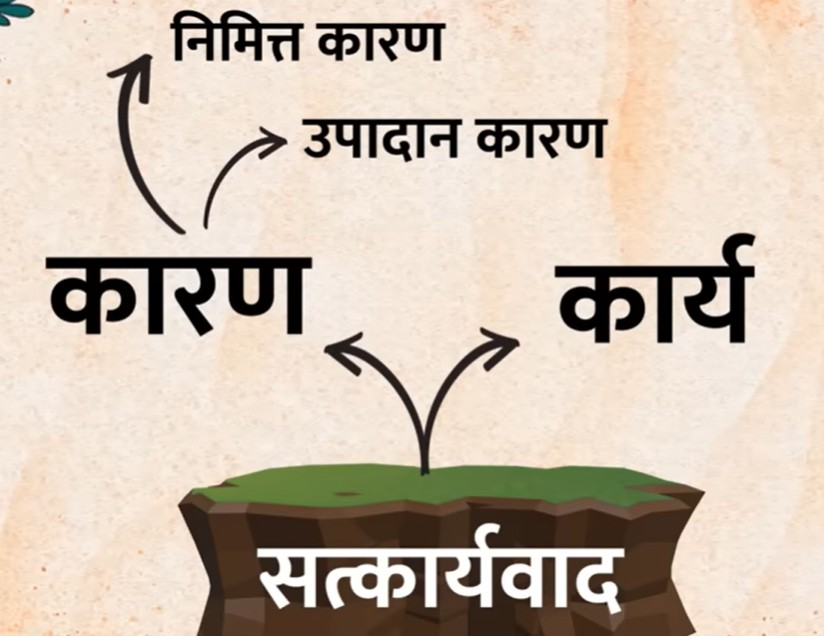
\includegraphics[width=\linewidth,keepaspectratio]{sankhya4}
		
		घड़े के लिए मिट्टी उपादान, कुम्हार निमित्त
		
        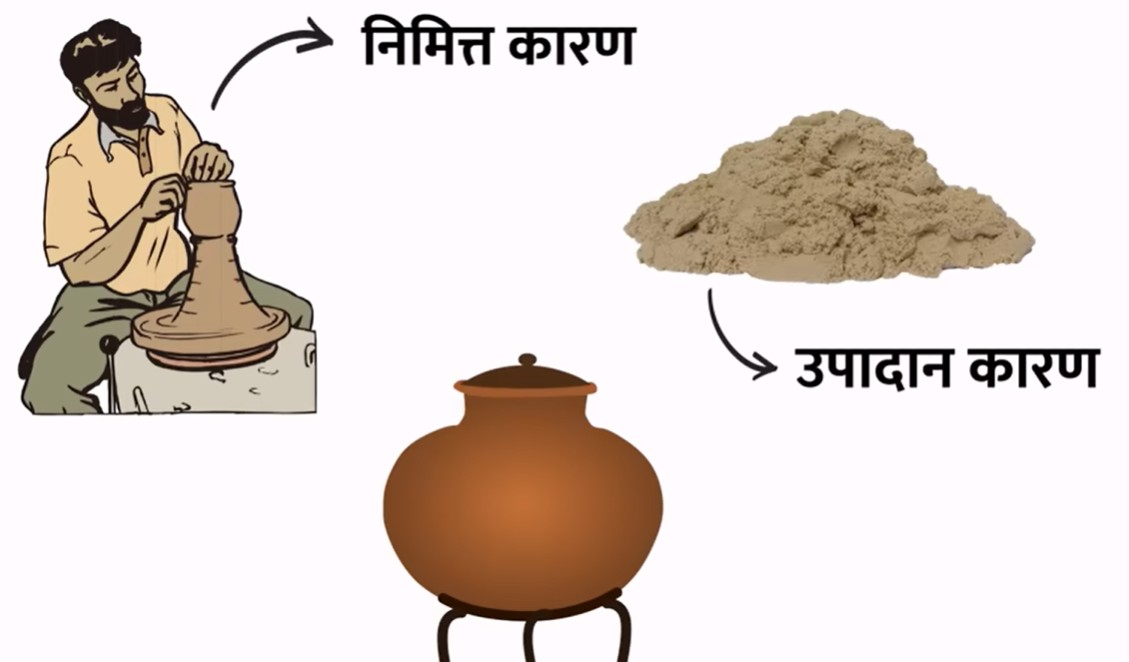
\includegraphics[width=\linewidth,keepaspectratio]{sankhya5}
		
		{\tiny (Ref: Samkhya Darshan - HyperQuest)}
		
      \end{center}	
    \end{column}
\end{columns}
\end{frame}

%%%%%%%%%%%%%%%%%%%%%%%%%%%%%%%%%%%%%%%%%%%%%%%%%%%%%%%%%%%
\begin{frame}[fragile]\frametitle{सृष्टि का प्रारंभ}
      \begin{itemize}
	\item सृष्टि की प्रक्रिया तब आरंभ होती है जब पुरुष और प्रकृति का सानिध्य होता है. यह कोई भौतिक संपर्क नहीं बल्कि एक प्रकार की निकटता या प्रभाव है.
	\item उदाहरण: चुंबक स्वयं निष्क्रिय होते हुए भी अपनी निकटता से लोहे में गति उत्पन्न करता है.
	\item चेतन पुरुष के सानिध्य मात्र से अचेतन प्रकृति में हलचल शुरू हो जाती है और प्रकृति के तीनों गुणों की साम्यावस्था भंग हो जाती है.
	\item यहीं से सृष्टि का विकास क्रम जिसे तत्व परिणाम कहा जाता है, शुरू होता है.
    \item कुल 25 तत्वों की गणना की जाती है – 2 मूल तत्व और 23 प्रकृति से उत्पन्न.
	  \end{itemize}
\end{frame}

%%%%%%%%%%%%%%%%%%%%%%%%%%%%%%%%%%%%%%%%%%%%%%%%%%%%%%%%%%%
\begin{frame}[fragile]\frametitle{२५ तत्त्व: सृष्टि का विकास क्रम}
\begin{itemize}
  \item \textbf{१. प्रकृति}: अव्यक्त मूल कारण.
  \item प्रकृति में असंतुलन होने पर पहला तत्व \textbf{२. महत या बुद्धि} उत्पन्न होता है. यह निर्णय और विवेक की शक्ति है.
  \item महत से \textbf{३. अहंकार} ('मैं' का भाव) उत्पन्न होता है. यह स्वयं को अलग अस्तित्व के रूप में अनुभव कराता है.
  \item अहंकार से विकास तीन दिशाओं में होता है:
  \begin{itemize}
    \item \textit{सात्विक अहंकार} से ११ तत्त्व उत्पन्न होते हैं:
      \begin{itemize}
        \item \textbf{४. मन}: संकल्प-विकल्प करने वाली वृत्ति.
        \item \textbf{५-९. पाँच ज्ञानेंद्रियां}: आँख, कान, नाक, जीभ, त्वचा.
        \item \textbf{१०-१४. पाँच कर्मेंद्रियां}: वाणी, हाथ, पाँव, गुदा, जननेंद्रिय.
      \end{itemize}
    \item \textit{तामसिक अहंकार} से उत्पन्न होते हैं:
      \begin{itemize}
        \item \textbf{१५-१९. पाँच तन्मात्राएं} (सूक्ष्म तत्व): शब्द, स्पर्श, रूप, रस, गंध के पोटेंशियल.
      \end{itemize}
  \end{itemize}
   \item पाँच तन्मात्राओं से ५ स्थूल भूत उत्पन्न होते हैं:
   \begin{itemize}
        \item \textbf{२०. आकाश} (शब्द से).
        \item \textbf{२१. वायु} (शब्द+स्पर्श से).
        \item \textbf{२२. अग्नि} (शब्द+स्पर्श+रूप से).
        \item \textbf{२३. जल} (शब्द+स्पर्श+रूप+रस से).
        \item \textbf{२४. पृथ्वी} (शब्द+स्पर्श+रूप+रस+गंध से).
    \end{itemize}
  \item अंतिम तत्त्व \textbf{२५. पुरुष} है, जो शुद्ध चेतन और अकर्ता है.
\end{itemize}
\end{frame}


%%%%%%%%%%%%%%%%%%%%%%%%%%%%%%%%%%%%%%%%%%%%%%%%%%%%%%%%%%%
\begin{frame}[fragile]\frametitle{बंधन एवं त्रिविध दुख}
      \begin{itemize}
	\item दुखों का मूल कारण है अविवेक, यानी पुरुष का प्रकृति और उसके विकारों (शरीर, मन, बुद्धि, अहंकार) से तादात्म्य.
	\item चेतना फंसकर अपने आप को प्रकृति समझने लगती है और अपना मूल स्वरूप भूल जाती है कि वह केवल साक्षी है. यह भ्रम ही दुख का मूल कारण है.
    \item मनुष्य जीवन में तीन प्रकार के दुखों से घिरा रहता है:
          \begin{itemize}
          \item \textbf{आध्यात्मिक दुख}: अपने शरीर और मन से उत्पन्न (रोग, चिंता, क्रोध, भय).
          \item \textbf{आधिभौतिक दुख}: अन्य प्राणियों या बाहरी वस्तुओं से मिलते हैं (जैसे गरीबी, अभाव).
          \item \textbf{आधिदैविक दुख}: प्राकृतिक या दैवी शक्तियों के कारण (बाढ़, भूकंप, तूफान).
          \end{itemize}
      \item सामान्य उपाय (दवाई, सुरक्षा, पूजा-पाठ) अस्थाई राहत देते हैं परंतु स्थाई समाधान नहीं.
      \end{itemize}
\end{frame}

%%%%%%%%%%%%%%%%%%%%%%%%%%%%%%%%%%%%%%%%%%%%%%%%%%%%%%%%%%%
\begin{frame}[fragile]\frametitle{मोक्ष का उपाय: विवेक ख्याति}
      \begin{itemize}
    \item सांख्य का परम लक्ष्य दुखों का अंत करना है.
	\item दुखों का जड़ से नाश तभी हो सकता है जब हमें उनका मूल कारण पता चले.
	\item मुक्ति का एकमात्र मार्ग है विवेक ख्याति – भेद ज्ञान. यह साधारण जानकारी नहीं, अनुभवजन्य ज्ञान है.
	\item जब यह बोध हो जाता है कि "मैं पुरुष इस शरीर-मन-बुद्धि से अलग शुद्ध चेतन सत्ता हूं", तब सारे दुख समाप्त हो जाते हैं.
    \item इसी अवस्था को मोक्ष या कैवल्य कहा जाता है.
	\item विवेक ज्ञान की प्राप्ति के उपाय:
        \begin{itemize}
            \item श्रवण (गुरु से सुनना), मनन (तर्कपूर्वक विचार), निदिध्यासन (ध्यान द्वारा चिंतन).
            \item योग दर्शन का अभ्यास, जिससे बुद्धि निर्मल होकर विवेक को प्रतिबिंबित करती है.
        \end{itemize}
	  \end{itemize}
\end{frame}

%%%%%%%%%%%%%%%%%%%%%%%%%%%%%%%%%%%%%%%%%%%%%%%%%%%%%%%%%%%
\begin{frame}[fragile]\frametitle{कैवल्य का क्रमिक पथ}
      \begin{itemize}
          \item जिस क्रम में चेतना प्रकृति में फंसी, उसी क्रम से वापस निकलना पड़ता है.
          \item \textbf{प्रथम चरण}: पंच महाभूत और तन्मात्राओं से मुक्ति. बाहरी विषयों (रूप, शब्द, गंध आदि) से परेशान न होना.
          \item \textbf{द्वितीय चरण}: इंद्रियों के दुख से मुक्ति. समझना कि आप अपनी इंद्रियां नहीं हैं, बल्कि चेतना हैं.
          \item \textbf{तृतीय चरण}: मन के दुख से मुक्ति. मन की चंचलता और भागदौड़ से बाहर निकलना. यह अवस्था अधिक कठिन होती है.
          \item \textbf{चतुर्थ चरण}: अहंकार की मुक्ति. यह अत्यंत कठिन है, "मैं" की व्यक्तिगत पहचान को छोड़ना पड़ता है.
          \item \textbf{पंचम चरण}: बुद्धि का त्याग. अंततः निर्णय करने वाली बुद्धि को भी भूलना पड़ता है. यह अंतिम और सबसे कठिन चरण है.
      \end{itemize}
\end{frame}

%%%%%%%%%%%%%%%%%%%%%%%%%%%%%%%%%%%%%%%%%%%%%%%%%%%%%%%%%%%
\begin{frame}[fragile]\frametitle{कैवल्य की अवस्था}
      \begin{itemize}
          \item सभी तत्वों से मुक्त होने पर चेतना को कैवल्य प्राप्त होता है. यह पुरुष का प्रकृति से पूर्ण पृथक्करण है.
          \item यह ब्रह्म में विलीन होना नहीं, स्वयं की शुद्ध चेतनता में स्थित होना है.
          \item व्यक्ति के सारे दुख पूर्णतः समाप्त हो जाते हैं और वह त्रिविध दुखों से पूर्णतः मुक्त हो जाता है.
          \item प्रकृति और पुरुष पूर्णतः अलग हो जाते हैं.
          \item प्रकृति भी समझ जाती है कि खेल समाप्त हो गया और वह मुक्त पुरुष के लिए अपना खेल समाप्त कर देती है.
          \item चेतना केवल रूप में स्थित हो जाती है - यही कैवल्य है.
      \end{itemize}
\end{frame}

%%%%%%%%%%%%%%%%%%%%%%%%%%%%%%%%%%%%%%%%%%%%%%%%%%%%%%%%%%%%%%%%%%%%%%%%%%%%%%%%%%
\begin{frame}[fragile]\frametitle{योग दर्शन से संबंध}
\begin{itemize}
  \item योग दर्शन सांख्य का ही व्यावहारिक रूप है.
  \item \textbf{पतंजलि योगसूत्र} में सांख्य के सिद्धांत आधार हैं.
  \item सांख्य – सिद्धांत; योग – अनुशासन, अभ्यास.
  \item सांख्य में विवेक का विकास होता है; योग में चित्तवृत्तियों का निरोध होता है.
  \item दोनों का लक्ष्य – \textbf{कैवल्य} / मोक्ष है.
  \item दोनों में 25 तत्त्वों की स्वीकृति समान है.
  \item सांख्य दर्शन ईश्वर को स्वीकार नहीं करता; योग दर्शन \textbf{ईश्वरप्रणिधान} को स्थान देता है.
\end{itemize}
\end{frame}

%%%%%%%%%%%%%%%%%%%%%%%%%%%%%%%%%%%%%%%%%%%%%%%%%%%%%%%%%%%%%%%%%%%%%%%%%%%%%%%%%%
\begin{frame}[fragile]\frametitle{अन्य दर्शनों से तुलना}
\begin{itemize}
  \item \textbf{वेदांत} – ब्रह्म को एक (अद्वैत) मानता है; सांख्य द्वैतवादी (प्रकृति+पुरुष) है.
  \item \textbf{बौद्ध} – अनात्मवाद (आत्मा नहीं) को मानता है; सांख्य अनेक आत्माएँ (पुरुष) मानता है.
  \item \textbf{न्याय-वैशेषिक} – तर्क और पदार्थ के आधार पर सृष्टि की व्याख्या करता है; सांख्य विवेक व प्रकृति के आधार पर करता है.
  \item \textbf{जैन दर्शन} – आत्मा और द्रव्य को अलग मानता है और कर्म बंधन से मुक्ति की बात करता है; सांख्य प्रकृति से भेद ज्ञान को ही मुक्ति मानता है.
\end{itemize}
\end{frame}

%%%%%%%%%%%%%%%%%%%%%%%%%%%%%%%%%%%%%%%%%%%%%%%%%%%%%%%%%%%%%%%%%%%%%%%%%%%%%%%%%%
\begin{frame}[fragile]\frametitle{वैज्ञानिक दृष्टिकोण एवं समकालीन उपयोगिता}
\begin{itemize}
  \item सांख्य दर्शन का विश्लेषणात्मक दृष्टिकोण आधुनिक विज्ञान से मेल खाता है.
  \item \textbf{सत्कार्यवाद} ऊर्जा/पदार्थ के संरक्षण के सिद्धांत जैसा है.
  \item \textbf{निष्क्रिय पुरुष, सक्रिय प्रकृति} – ऑब्जर्वर थेओरी (Observer Effect) से संबंधित हो सकता है.
  \item \textbf{विवेकज्ञान} को मेटा-कॉग्निशन (Self-awareness) से जोड़ा जा सकता है.
  \item मानसिक स्वास्थ्य में त्रिगुण सिद्धांत का प्रयोग होता है.
  \item यह आत्मनिरीक्षण, mindfulness, योग और ध्यान का मूल आधार है.
\end{itemize}
\end{frame}

%%%%%%%%%%%%%%%%%%%%%%%%%%%%%%%%%%%%%%%%%%%%%%%%%%%%%%%%%%%%%%%%%%%%%%%%%%%%%%%%%%
\begin{frame}[fragile]\frametitle{निष्कर्ष – सांख्य दर्शन का सार}
\begin{itemize}
  \item दो स्वतंत्र तत्त्व हैं – \textbf{प्रकृति} और \textbf{पुरुष}.
  \item सृष्टि – प्रकृति द्वारा पुरुष के लिए अनुभव का एक माध्यम है.
  \item दुःख – अविवेक से उत्पन्न होता है; मोक्ष – विवेक से प्राप्त होता है.
  \item मोक्ष का अर्थ – प्रकृति से पुरुष का पूर्ण वैराग्य और अपने शुद्ध स्वरूप में स्थित होना है.
  \item यह अत्यंत तर्कसंगत, विज्ञानसम्मत एवं अनुभवशील दर्शन है.
  \item चेतना का प्रकृति में फंसना और वापस मुक्त होना ही संख्या दर्शन है.
  \item यह संपूर्ण दर्शन आत्म-साक्षात्कार और मुक्ति का मार्ग दिखाता है.
\end{itemize}
\end{frame}